\documentclass[conference]{IEEEtran}
\IEEEoverridecommandlockouts
\usepackage{cite}
\usepackage{amsmath,amssymb}
\usepackage{graphicx}
\usepackage{booktabs}
\usepackage{multirow}
\usepackage{algorithm}
\usepackage{algpseudocode}
\usepackage{tikz}
\usetikzlibrary{arrows.meta,positioning,fit}
\usepackage{xcolor}
\usepackage{url}
\usepackage{pifont}
\newcommand{\cmark}{\ding{51}}
\newcommand{\xmark}{\ding{55}}
\graphicspath{{fig/}}
\algrenewcommand\algorithmicrequire{\textbf{Input:}}
\algrenewcommand\algorithmicensure{\textbf{Output:}}

\begin{document}

\title{Trust or Measure? Confidence-Gated CPU--GPU Execution Selection}

\author{\begin{tabular}[t]{@{}c@{}}Srivathsa B S\\[3pt]\footnotesize\textit{Manipal Institute of Technology, Bengaluru}\\\footnotesize\textit{Manipal Academy of Higher Education}\\\footnotesize Manipal, India\end{tabular}
\hfill
\begin{tabular}[t]{@{}c@{}}Manas Verma\\[3pt]\footnotesize\textit{Manipal Institute of Technology, Bengaluru}\\\footnotesize\textit{Manipal Academy of Higher Education}\\\footnotesize Manipal, India\end{tabular}
\hfill
\begin{tabular}[t]{@{}c@{}}Pavithra N\\[3pt]\footnotesize\textit{Manipal Institute of Technology, Bengaluru}\\\footnotesize\textit{Manipal Academy of Higher Education}\\\footnotesize Manipal, India\end{tabular}}
\maketitle

\begin{abstract}
Most practitioners send machine learning work to the GPU out of habit. On a single laptop with an RTX~3050 and an eight-core Ryzen CPU, we found that habit wrong below a size threshold for seven of ten common PyTorch operations, and wrong at every size we measured for one of them (FFT). This paper reports what we learned building and measuring AutoHetero, a runtime layer that predicts, per call, whether a workload should run on the CPU, the GPU, or both, and that rebalances mid-call when the GPU falls behind. We use its measurements to test, one by one, the claims behind a proposed confidence-gated execution strategy selector. A random-forest predictor picked the faster device for 91.1\% of unseen input sizes but only 68.8\% of unseen operation types. A confidence score built from tree disagreement, which we evaluate offline, separated right from wrong decisions well on familiar operations: measuring only the 5.6\% of least-confident cases lifted accuracy from 91.1\% to 96.0\%. On unfamiliar operations the same score was confidently wrong, at 14\% accuracy and 0.84 median confidence for FFT. Monitoring every call cost AutoHetero about 30\% against always-GPU on an idle machine, and a decision trained idle failed badly under CPU contention (0.21$\times$). Splitting work across both devices rarely paid. Taken together, the results back measuring only when unsure, but they show that tree spread alone cannot tell the selector when it is unsure.
\end{abstract}

\begin{IEEEkeywords}
heterogeneous computing, CPU--GPU scheduling, performance prediction, random forest, confidence estimation, selective calibration, runtime systems
\end{IEEEkeywords}

% ---------------------------------------------------------------------------
\section{Introduction}

CPUs and GPUs are built for different work. A CPU has a few fast, flexible cores that handle branching, step-by-step logic well. A GPU has thousands of simple cores that apply one operation to a great deal of data at once, but every job pays a setup cost first: a kernel launch, and usually a copy of the inputs across PCIe. Neither processor is faster in general. Which one wins depends on the input size, the arithmetic per byte, and how much data has to move.

In practice the choice is made by hand, and the default is ``use the GPU.'' We think the default survives because its failures are quiet. A small job sent to the GPU still finishes; it just finishes later than it would have on the CPU, and nobody times the alternative. Four situations make the habit expensive: small inputs, where launch and copy costs exceed the compute saved; heavy data movement, where host-to-device transfers add time the kernel never wins back; a shared GPU, where jobs compete for cores, memory and bandwidth; and over-concurrency, where past some point more parallel jobs slow every job down.

Our proposed project, \emph{Intelligent Execution Strategy Selection}, targets this choice for whole jobs on a CPU--GPU server. Given a workload that can run on either device, it should pick the strategy (CPU, GPU, both, or $N$ concurrent GPU processes under NVIDIA MPS) that minimises execution time, without exhaustively trying every option. Three ideas set it apart from prior work: choosing the device and the GPU concurrency level as one decision; attaching a confidence score to every prediction; and measuring before committing \emph{only} when that confidence is low.

Before building that system, we built a smaller one. AutoHetero makes the same kind of decision per function call inside one Python program. It has no concurrency decision and no confidence score, but it does predict device times with random forests, it measures some calls on both devices, and it was evaluated on a fixed machine against always-CPU, always-GPU and a per-run oracle. Its data can therefore test several of the proposal's premises directly and one of its mechanisms offline.

That is what this paper does. Our contributions are:
\begin{itemize}
\item the design of AutoHetero, a zero-configuration dispatcher with per-machine calibration, a log-time random-forest predictor, chunked execution and a slowdown-triggered CPU+GPU rebalance (Section~\ref{sec:system});
\item a measured evaluation on one fixed laptop across ten operations and four load conditions, with every dispatcher overhead charged (Sections~\ref{sec:setup}--\ref{sec:results});
\item an offline test of confidence-gated selection on the same data, using agreement between per-device trees as the confidence score (Section~\ref{sec:confidence});
\item a claim-by-claim map from the proposal to the evidence, stating which claims the data supports, which it contradicts, and which it cannot reach (Section~\ref{sec:map}).
\end{itemize}

One boundary needs saying up front. AutoHetero's results support only what AutoHetero measured. They can motivate the proposal's claims or warn against them, but they do not replace the measurements the proposal itself must make, and nothing here measures MPS concurrency.

% ---------------------------------------------------------------------------
\section{Background and Related Work}
\label{sec:related}

Qilin~\cite{qilin} splits one program's work between CPU and GPU by fitting a performance model from training runs, the ``measure a little, predict the rest'' idea we reuse as per-machine calibration. Its weakness is that the training runs happen for every new program, however certain the outcome. Grewe and O'Boyle~\cite{grewe11} predict the best split from static code features alone; their later work makes the mapping portable across devices~\cite{grewe13}. Static features cannot see input size, though, and Kofler et al.~\cite{kofler} show that the right partition depends on it. Pai et al.~\cite{pai} find that running GPU kernels concurrently often gains little over running them one after another, so the concurrency level has to be chosen rather than maximised; they assume the GPU is the right device to begin with. Hayat et al.~\cite{hayat} learn a resource-efficient task-to-resource mapping on heterogeneous systems. StarPU~\cite{starpu} schedules tasks across heterogeneous units using history-based performance models, and ONNX Runtime~\cite{onnxrt} lets the user pick an execution provider by hand.

Table~\ref{tab:gap} places these against four properties. Each building block exists. What none of the surveyed work does is choose the device and the GPU concurrency together while also deciding, per job, whether its own prediction is trustworthy enough to skip measurement.

\begin{table}[t]
\centering
\caption{Coverage of the four properties in the surveyed work}
\label{tab:gap}
\setlength{\tabcolsep}{2.5pt}
\begin{tabular}{@{}lcccc@{}}
\toprule
Work & Device & Input-size & GPU & Selective \\
     & choice & aware & concurrency & calibration \\
\midrule
Qilin~\cite{qilin} & \cmark & \cmark & \xmark & \xmark \\
Grewe~\cite{grewe11} & \cmark & \xmark & \xmark & \xmark \\
Kofler et al.~\cite{kofler} & \cmark & \cmark & \xmark & \xmark \\
Pai et al.~\cite{pai} & \xmark & \xmark & \cmark & \xmark \\
AutoHetero (here) & \cmark & \cmark & \xmark & partial$^{a}$ \\
Proposed selector & \cmark & \cmark & \cmark & \cmark \\
\bottomrule
\end{tabular}\\[2pt]
\footnotesize{$^{a}$Measures every splittable call in chunks; confidence gating evaluated offline only.}
\end{table}

% ---------------------------------------------------------------------------
\section{AutoHetero: System Design}
\label{sec:system}

AutoHetero is a Python library over PyTorch. A user enables it with one line, or marks a function with \texttt{@autohetero.auto}; inputs may be tensors or NumPy arrays and come back in the type and on the device they arrived in. Fig.~\ref{fig:arch} shows the path of a call.

\begin{figure}[t]
\centering
\resizebox{\columnwidth}{!}{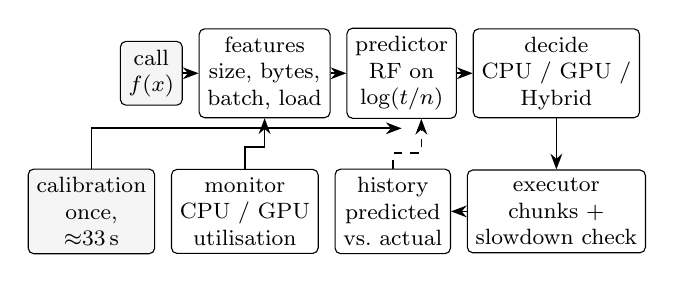
\begin{tikzpicture}[
  box/.style={draw, rounded corners=2pt, align=center, font=\footnotesize, minimum height=0.7cm, inner sep=3pt},
  arr/.style={-{Stealth[length=2mm]}, semithick},
  node distance=0.2cm]
\node[box, fill=gray!8] (call) {call\\$f(x)$};
\node[box, right=of call] (feat) {features\\size, bytes,\\batch, load};
\node[box, right=of feat] (pred) {predictor\\RF on\\$\log(t/n)$};
\node[box, right=of pred] (dec) {decide\\CPU / GPU /\\Hybrid};
\node[box, below=0.65cm of dec] (exec) {executor\\chunks +\\slowdown check};
\node[box, left=of exec] (hist) {history\\predicted\\vs.\ actual};
\node[box, left=of hist] (mon) {monitor\\CPU / GPU\\utilisation};
\node[box, left=of mon, fill=gray!8] (cal) {calibration\\once,\\$\approx$33\,s};
\draw[arr] (call) -- (feat);
\draw[arr] (feat) -- (pred);
\draw[arr] (pred) -- (dec);
\draw[arr] (dec) -- (exec);
\draw[arr] (exec) -- (hist);
\draw[arr] (mon.north) -- ++(0,0.28) -| (feat.south);
\draw[arr] (cal.north) |- ([yshift=-0.12cm]pred.south west) -- ([yshift=-0.12cm]pred.south);
\draw[arr, dashed] (hist.north) -- ++(0,0.2) -| ([xshift=0.25cm]pred.south);
\end{tikzpicture}}
\caption{The path of one dispatched call. Calibration trains the predictor once per machine; every measured call is logged with its prediction and feeds later retraining (dashed).}
\label{fig:arch}
\end{figure}

\subsection{Calibration and features}

On first use, AutoHetero times each built-in operation on the CPU and the GPU at roughly six log-spaced sizes, together with host-to-device bandwidth, device-to-host bandwidth and kernel launch latency. On the evaluation laptop this took 32.6\,s and measured 6.4\,GB/s to the GPU, 3.4\,GB/s back, and 65\,\textmu s per launch. Results are cached under a key built from the CPU model, GPU name, driver and PyTorch version, so a driver update triggers recalibration.

A call is described by a feature vector $\mathbf{x}$: total input elements $n$, input bytes, batch size, bytes per element, current CPU and GPU utilisation from a background sampler (read from a cache, so no system call sits on the hot path), and a one-hot operation identifier.

\subsection{Prediction}

For each device $d \in \{\mathrm{cpu}, \mathrm{gpu}\}$ we train a random forest~\cite{breiman} $F_d$ of 100 regression trees~\cite{sklearn} on the target $y = \log(t/n)$, the log of seconds per input element. Predicted time is then $\hat t_d(\mathbf{x}) = n\,\exp F_d(\mathbf{x})$.

The choice of target matters more than it looks. Raw time spans five orders of magnitude here, and a model fitted to it is dominated by the largest jobs, yet the small jobs are precisely where the CPU wins. The log fixes that. Dividing by $n$ fixes a second problem: a forest cannot extrapolate, so a forest on log time would predict a flat time beyond the largest calibrated size. On seconds per element, its flat extrapolation becomes a linear one in time.

A forest prediction takes about 27\,ms on this laptop, which is far too slow to pay on every call. AutoHetero caches decisions keyed on the operation, $\lfloor \log_2 n \rfloor$, data type and a 25\%-wide load bucket, and runs the forests only on a cache miss.

For splittable calls, a CPU+GPU split (``Hybrid'') competes with the single devices. If both devices run their share concurrently and finish together, the ideal time is
\begin{equation}
\hat t_{\mathrm{hyb}} = \frac{\hat t_{\mathrm{cpu}}\,\hat t_{\mathrm{gpu}}}{\hat t_{\mathrm{cpu}} + \hat t_{\mathrm{gpu}}} + c_{\mathrm{split}},
\label{eq:hybrid}
\end{equation}
where $c_{\mathrm{split}}$ (thread start plus concatenation) is measured during calibration. The GPU receives the share $\hat t_{\mathrm{cpu}}/(\hat t_{\mathrm{cpu}}+\hat t_{\mathrm{gpu}})$ of the batch. Hybrid is chosen only if it beats the faster single device by a 10\% margin. Algorithm~\ref{alg:decide} summarises the decision.

\begin{algorithm}[t]
\caption{Per-call device decision in AutoHetero}
\label{alg:decide}
\begin{algorithmic}[1]
\Require call features $\mathbf{x}$, forests $F_{\mathrm{cpu}}, F_{\mathrm{gpu}}$, cache $C$, splittable flag $s$
\Ensure mode $m \in \{\mathrm{cpu}, \mathrm{gpu}, \mathrm{hybrid}\}$ and predicted times $\hat{\mathbf{t}}$
\State $k \gets (\mathrm{op}, \lfloor\log_2 n\rfloor, \mathrm{dtype}, \mathrm{load\ bucket}, s)$
\If{$k \in C$} \State \Return $C[k]$ \Comment{$\approx$0.16\,ms path}
\EndIf
\For{$d \in \{\mathrm{cpu}, \mathrm{gpu}\}$}
  \State $\hat t_d \gets n \cdot \exp F_d(\mathbf{x})$ \Comment{$\approx$27\,ms path}
\EndFor
\State $m \gets \arg\min_d \hat t_d$
\If{$s$ \textbf{and} batch $>1$}
  \State compute $\hat t_{\mathrm{hyb}}$ by \eqref{eq:hybrid}
  \If{$\hat t_{\mathrm{hyb}} < 0.9\,\hat t_m$} $m \gets \mathrm{hybrid}$ \EndIf
\EndIf
\State $C[k] \gets (m, \hat{\mathbf{t}})$; \Return $(m, \hat{\mathbf{t}})$
\end{algorithmic}
\end{algorithm}

\subsection{Chunked execution and rebalancing}

A prediction made before a call cannot see a GPU that becomes busy during it. For splittable calls above a minimum size, AutoHetero therefore runs the batch in chunks of about 10\% (each at least 5\,ms, since shorter chunks are dominated by launch overhead) and compares each chunk's time with its prediction. If a chunk runs more than $1.5\times$ slower than predicted, the rest of the call switches to Hybrid, split by the speeds just measured and re-split after every round (Algorithm~\ref{alg:chunk}). Two threads feed the devices; PyTorch releases the global interpreter lock inside its operators, so both run at once. Functions written by the user have no calibration data, so their first splittable call runs one chunk on each device as a trial and fits a per-function log--log model from then on.

\begin{algorithm}[t]
\caption{Chunked execution with slowdown-triggered rebalance}
\label{alg:chunk}
\begin{algorithmic}[1]
\Require batch of $B$ items, chosen device $d$, per-piece predictor $\hat t_\cdot(\cdot)$
\State $c \gets \max(\lceil 0.1B\rceil,\ \text{items filling } 5\,\mathrm{ms})$; $i \gets 0$
\While{$i < B$}
  \State run items $[i, i{+}c)$ on $d$, measuring $t$; $i \gets i + c$
  \If{not first chunk \textbf{and} $t > 1.5\,\hat t_d(c)$}
    \State $v_{\mathrm{cpu}}, v_{\mathrm{gpu}} \gets$ measured or predicted speeds
    \While{$i < B$} \Comment{Hybrid rounds of $\approx$25\%}
      \State $r \gets$ next round; $g \gets \lceil r\,v_{\mathrm{gpu}}/(v_{\mathrm{cpu}}+v_{\mathrm{gpu}})\rceil$
      \State run $g$ on GPU $\parallel$ $r{-}g$ on CPU; update $v$
      \State $i \gets i + r$
    \EndWhile
  \EndIf
\EndWhile
\State concatenate pieces in original order
\end{algorithmic}
\end{algorithm}

Only functions marked splittable, whose output rows depend only on the matching input rows, are chunked. Splitting \texttt{sort} or \texttt{groupby} would silently give wrong answers, and we would rather lose speed than correctness. Any GPU error (no CUDA, out of memory, a driver fault) reruns the call on the CPU.

% ---------------------------------------------------------------------------
\section{Confidence-Gated Selection}
\label{sec:confidence}

AutoHetero measures much of the time: every chunk of every long splittable call is checked against its prediction. The proposal argues for the opposite policy. Trust the prediction when the model is sure, and measure a few candidates only when it is not. To test that on AutoHetero's data we need a confidence score, and the proposal names one: disagreement across the trees of the forest.

The decision is a comparison of two forests, so we define confidence through their trees jointly. Let $f^{(i)}_{\mathrm{cpu}}$ and $f^{(j)}_{\mathrm{gpu}}$ be the $i$-th and $j$-th trees ($T = 100$ each). Both predict $\log(t/n)$ for the same $n$, so comparing them compares times directly. The share of tree pairs that vote for the CPU is
\begin{equation}
p_{\mathrm{cpu}}(\mathbf{x}) = \frac{1}{T^2}\sum_{i=1}^{T}\sum_{j=1}^{T} \mathbf{1}\!\left[f^{(i)}_{\mathrm{cpu}}(\mathbf{x}) < f^{(j)}_{\mathrm{gpu}}(\mathbf{x})\right],
\label{eq:conf}
\end{equation}
and the confidence of the forests' pick $m$ is $\kappa = p_{\mathrm{cpu}}$ if $m = \mathrm{cpu}$ and $1 - p_{\mathrm{cpu}}$ otherwise. A value of 1 means every pair agrees with the pick; 0.5 is a coin toss. Because the pick comes from the forest means and $\kappa$ from pairwise votes, $\kappa$ can fall slightly below 0.5.

Algorithm~\ref{alg:gate} is the gating rule. In the offline evaluation, ``measure'' means taking the measured winner of the two devices, and the probe itself is charged at zero. The regrets we report for it are therefore lower bounds; what a probe really costs is a question only the proposed system's own measurements can answer.

\begin{algorithm}[t]
\caption{Confidence-gated strategy selection (evaluated offline)}
\label{alg:gate}
\begin{algorithmic}[1]
\Require features $\mathbf{x}$, per-device forests, threshold $\tau$
\State $m \gets \arg\min_d \hat t_d(\mathbf{x})$; compute $\kappa$ from \eqref{eq:conf}
\If{$\kappa \ge \tau$}
  \State \Return $m$ \Comment{trust: no measurement}
\Else
  \State run a short probe of each candidate strategy
  \State \Return the measured winner \Comment{log result for retraining}
\EndIf
\end{algorithmic}
\end{algorithm}

% ---------------------------------------------------------------------------
\section{Experimental Setup}
\label{sec:setup}

\textbf{Machine.} All final numbers come from one fixed laptop: AMD Ryzen~7 5800H (8 cores, 16 threads), NVIDIA RTX~3050 Laptop GPU (4\,GB, 60\,W), 16\,GB RAM, Windows, PyTorch~2.11 with CUDA~12.8~\cite{pytorch}. We used cloud notebooks only during development, because their GPUs and background load change from session to session.

\textbf{Workloads.} Ten PyTorch operations, each with a single code path that runs on either device (Table~\ref{tab:workloads}), plus one user-defined image-enhancement function. The two networks use random weights with a fixed seed.

\begin{table}[t]
\centering
\caption{Workloads and the crossover each one showed}
\label{tab:workloads}
\setlength{\tabcolsep}{3pt}
\begin{tabular}{@{}llrr@{}}
\toprule
Domain & Op & CPU faster up to & $T_{cpu}/T_{gpu}$ range \\
 & & (elements) & \\
\midrule
\multirow{3}{*}{Image} & blur & 786\,432 & 0.68--4.15 \\
 & resize & 786\,432 & 0.50--1.55 \\
 & sobel & 196\,608 & 0.78--7.91 \\
\multirow{2}{*}{Inference} & resnet18 & never & 1.28--19.5 \\
 & mobilenetv2 & never & 1.55--13.2 \\
\multirow{3}{*}{Analytics} & filter & 1\,264\,912 & 0.18--1.16 \\
 & sort & 4\,000 & 0.50--37.7 \\
 & groupby & 6\,324 & 0.20--21.6 \\
\multirow{2}{*}{Scientific} & matmul & 131\,072 & 0.12--9.34 \\
 & fft & always & 0.44--0.89 \\
\bottomrule
\end{tabular}
\end{table}

\textbf{Protocol.} Every workload, size and device was run five times after one discarded warm-up, timed with transfers included and with \texttt{torch.cuda.synchronize()} before any GPU timer stopped. This gave a dataset of 124 sizes measured on both devices.

\textbf{Conditions.} Idle; GPU stress (a second PyTorch process on the GPU, time-sliced, without MPS); CPU stress (Python busy loops on every core, since \texttt{stress-ng} was unavailable on Windows); and battery power.

\textbf{Baselines and metrics.} Always-CPU, always-GPU, and an oracle that takes the best measured option in each run. We report geometric-mean speed-up, the share of workloads within 5\% of the oracle, decision accuracy (share of sizes where the predicted faster device was the measured faster one), regret (extra time from following predictions instead of the oracle), and per-call overhead. All of AutoHetero's own costs (features, prediction, trials, chunking) are inside every AutoHetero number.

% ---------------------------------------------------------------------------
\section{Results}
\label{sec:results}

\subsection{The right device depends on input size}

Fig.~\ref{fig:crossover} plots $T_{cpu}/T_{gpu}$ against input size; points below the dashed line are sizes where the CPU won. For seven of the ten operations the winner flips with size. The flip comes early for data-dependent work (sort and groupby cross over at a few thousand elements, after which the GPU is up to $37.7\times$ faster) and late for light, memory-bound work (filter only breaks even at about $10^6$ rows and never gains much). The two networks favoured the GPU at every batch, by up to $19.5\times$.

FFT is the outlier. The CPU won at every size we measured, with the GPU managing only 0.44--0.89 of its speed. For that operation, ``use the GPU'' is wrong without exception.

\begin{figure*}[t]
\centering
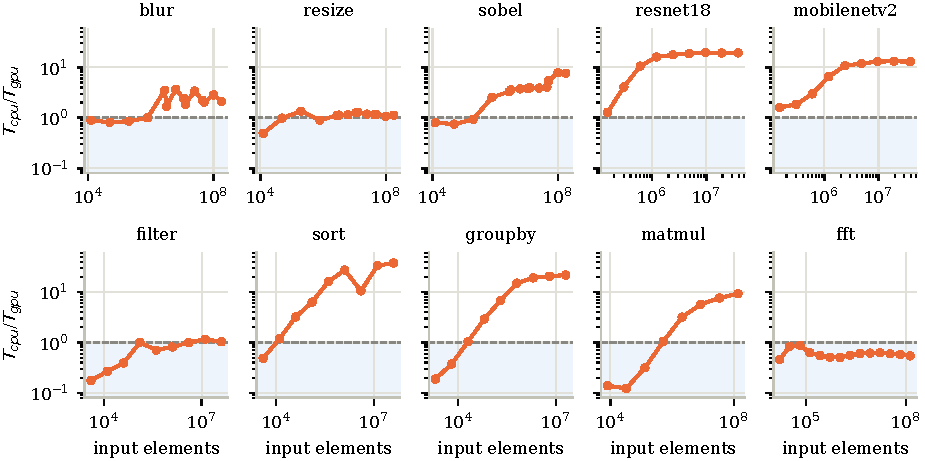
\includegraphics[width=\textwidth]{crossover}
\caption{GPU speed-up over the CPU against input elements (log--log, median of five runs). Shaded region: the CPU is faster. Seven operations cross over; resnet18 and mobilenetv2 never favour the CPU; fft never favours the GPU.}
\label{fig:crossover}
\end{figure*}

\subsection{Prediction accuracy, seen and unseen}

Fig.~\ref{fig:rq1} reports decision accuracy. On sizes held out from operations it had seen, the forest picked the faster device 91.1\% of the time under 5-fold cross-validation (regret 4.3\%) and 88\% on an 80/20 split. The model AutoHetero actually ships, trained only on the 33-second calibration, reached 80.7\%.

The figure that matters for the proposal is the third bar. Holding out a whole operation, accuracy fell to 68.8\% for the forest (74.4\% for a single tree, though with 36\% regret against the forest's 16\%). And the errors were not spread evenly. FFT, the operation least like the others, scored 14\%: having learned that large inputs favour the GPU, the model kept saying so.

\begin{figure}[t]
\centering
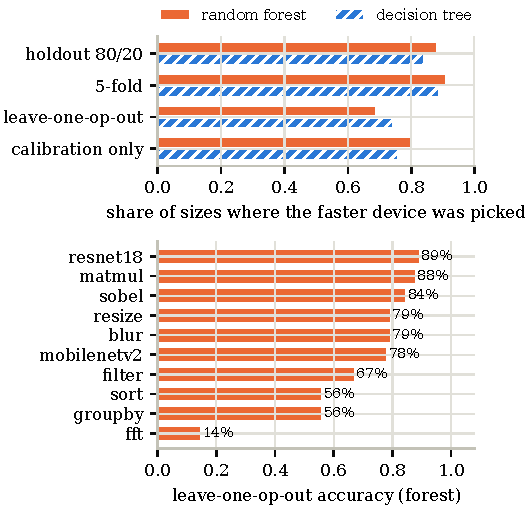
\includegraphics[width=\columnwidth]{rq1}
\caption{Top: decision accuracy by evaluation. Bottom: accuracy of the forest on each operation when that operation is left out of training.}
\label{fig:rq1}
\end{figure}

\subsection{Does tree disagreement know when it is wrong?}

We recomputed the forests on the development machine, pooling every held-out size, and scored $\kappa$ for each prediction. Under 5-fold cross-validation the answer is yes. The median confidence of correct decisions was 0.92 against 0.48 for wrong ones, which is about as clean a separation as one could ask for. Measuring only the sizes below $\tau = 0.5$ (5.6\% of them) raised pooled accuracy from 91.1\% to 96.0\% and removed almost all pooled regret (4.1\% to under 0.1\%). Measuring 21.8\% reached 99.2\% (Fig.~\ref{fig:confidence}, left).

Under leave-one-op-out the answer is no, and that surprised us. Correct and wrong decisions had nearly identical median confidence, 0.69 and 0.73, so the wrong ones were if anything slightly \emph{more} confident. Fig.~\ref{fig:confidence} (right) shows why: FFT sits in the bottom right, 14\% accurate at a median confidence of 0.84. Every tree had learned the same pattern from the other nine operations, so they agreed, and they agreed on the wrong answer. To push held-out accuracy past 93\% the gate had to measure 82\% of sizes, which is little better than measuring everything.

The lesson is narrow but, we think, important. Tree disagreement measures uncertainty \emph{within} the training distribution. It does not detect that a job lies outside it. A selector that relies on it alone will be most confident on precisely the jobs it has never seen.

\begin{figure}[t]
\centering
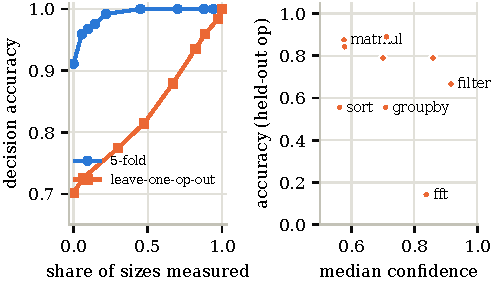
\includegraphics[width=\columnwidth]{confidence}
\caption{Left: accuracy as more of the least-confident sizes are measured (thresholds $\tau = 0, 0.5, \ldots, 1$). Right: per held-out operation, median confidence against accuracy.}
\label{fig:confidence}
\end{figure}

\subsection{End-to-end: AutoHetero against fixed strategies}

Fig.~\ref{fig:rq2} compares AutoHetero with always-GPU on each workload. We leave out sort at $10^7$ rows: its forced-GPU run always came right after a 3.4\,s CPU sort and took 260--270\,ms, while the same GPU sort run alone took about 91\,ms.

AutoHetero was faster than always-CPU in every condition (geometric means of $2.90\times$ idle, $2.00\times$ under GPU stress, $1.50\times$ under CPU stress, $2.57\times$ on battery). Against always-GPU it lost in every condition: $0.70\times$, $0.82\times$, $0.21\times$ and $0.65\times$. It came within 5\% of the oracle on only 4 of 17, 6 of 16, 4 of 15 and 4 of 16 workloads.

Three failure modes account for most of the gap. One is the cost of watching. Idle, with nothing to react to, chunking and checking every splittable call cost about 30\%, and the slowdown switch still fired in 10\% of runs (80\% for FFT at 4096). Another is switching onto a loaded device. Under CPU stress, GPU chunks looked slow, so the rule moved the remaining work to Hybrid, which put half of it on the busy CPU: resnet18 at batch 128 took 8.97\,s against 0.37\,s on the GPU alone. The third is the optimistic Hybrid estimate, covered next.

Contention itself was real. With one time-sliced neighbour on the GPU, GPU-only runs took $1.68\times$ as long (range 1.2--2.3$\times$ over 16 workloads). Under that stress the switch fired in 34\% of runs and detected the slowdown in a median 74\,ms, but it paid off on few workloads (mobilenetv2 at batch 128 gained 1.20$\times$).

\begin{figure}[t]
\centering
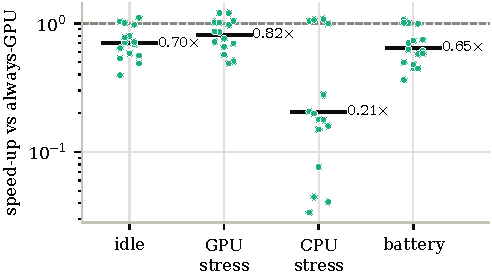
\includegraphics[width=\columnwidth]{rq2}
\caption{AutoHetero's speed-up over always-GPU per workload (dots) and geometric mean (bar), by load condition. Below the dashed line AutoHetero was slower.}
\label{fig:rq2}
\end{figure}

\subsection{Splitting across both devices}

Equation~\eqref{eq:hybrid} promises that a split finishes sooner than either device alone. On this machine it rarely did (Fig.~\ref{fig:hybrid}). Hybrid beat GPU-only only for resize at batch 256 (+11\%), filter at $10^7$ rows (+1\%) and mobilenetv2 at batch 2 (+19\%). Even at their best batch, resnet18 lost 64\%, sobel 77\%, blur 22\%, matmul 17\% and FFT 10\%. The estimate also misled the decision: AutoHetero chose Hybrid for mobilenetv2 at batch 32, which took 165\,ms against 60\,ms on the GPU.

We suspect two causes, though we did not isolate either. The CPU is not idle in GPU mode, since it launches kernels and moves data, so giving it real work slows the GPU's feeder. And on a laptop both chips share one power and thermal budget. Pipelining is also absent: each chunk is copy, compute, synchronise, in sequence, so transfers never overlap compute.

\begin{figure}[t]
\centering
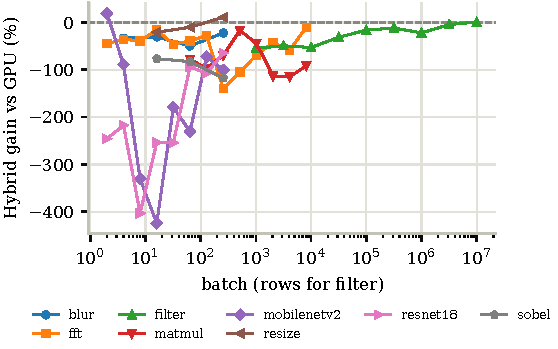
\includegraphics[width=\columnwidth]{hybrid}
\caption{Gain of a CPU+GPU split over GPU-only, by batch size, on the idle machine. Almost every point lies below zero.}
\label{fig:hybrid}
\end{figure}

\subsection{Overhead}

Table~\ref{tab:overhead} lists the per-call cost. A cached decision costs 0.16\,ms and a user function 0.10\,ms, both under the 1\,ms we had budgeted. An uncached forest decision costs 26.9\,ms, which is why AutoHetero needs its cache. For whole jobs lasting seconds the same 27\,ms is negligible, so the proposed selector can afford to run its model on every job; the 33\,s calibration is the larger one-off cost.

\begin{table}[t]
\centering
\caption{Dispatch overhead per call}
\label{tab:overhead}
\begin{tabular}{@{}lr@{}}
\toprule
Case & Cost \\
\midrule
Direct call, no AutoHetero & 0.14\,\textmu s \\
\texttt{@auto} function & 96.8\,\textmu s \\
\texttt{@auto} function, NumPy input & 136.3\,\textmu s \\
Built-in op, cached decision & 157.9\,\textmu s \\
Decision miss (forests run) & 26.9\,ms \\
Calibration, once per machine & 32.6\,s \\
\bottomrule
\end{tabular}
\end{table}

% ---------------------------------------------------------------------------
\section{Mapping the Evidence to the Proposal's Claims}
\label{sec:map}

Table~\ref{tab:map} lines up each claim from the proposal with what AutoHetero measured. Most premises hold. The two mechanisms the proposal depends on most, confidence and selective measurement, are supported in direction and weakened in detail.

\begin{table*}[t]
\centering
\caption{Proposal claims against AutoHetero's measurements}
\label{tab:map}
\renewcommand{\arraystretch}{1.12}
\begin{tabular}{@{}p{3.7cm}p{6.8cm}p{3.4cm}l@{}}
\toprule
Claim & AutoHetero evidence & Implication & Verdict \\
\midrule
The best device depends on the workload; small jobs and data movement make the GPU lose &
CPU faster below a crossover for 7/10 ops; GPU always faster for two networks; CPU always faster for FFT (Fig.~\ref{fig:crossover}) &
Input size must be a feature & Supported \\
Jobs sharing one GPU compete &
One time-sliced neighbour: GPU-only time $1.68\times$ (1.2--2.3$\times$) &
Motivates choosing concurrency; says nothing about MPS & Motivation only \\
One GPU, no competing users can be assumed &
Idle-trained decisions: $0.21\times$ always-GPU under CPU stress &
Main threat on shared servers; make decisions load-aware & Risky \\
A model trusted blindly fails on unfamiliar jobs &
91.1\% on unseen sizes vs.\ 68.8\% on unseen ops; FFT 14\% &
Case for confidence and held-out testing & Supported \\
Tree disagreement gives the confidence score &
Separates right/wrong in-distribution (0.92 vs.\ 0.48); fails on unseen ops (0.69 vs.\ 0.73) &
Add a novelty check; measure unseen job types first & Partly supported \\
Measure only when unsure; calibrate a minority of jobs &
Always-on monitoring cost $\approx$30\% idle; gating 5.6\% of familiar sizes: 91.1$\to$96.0\% &
Gate works for familiar jobs only & Supported, with limits \\
A simple CPU+GPU ratio split suffices &
Hybrid won on 3 of 8 ops, at most +19\%; ideal-overlap estimate over-promised &
Choose CPU+GPU only after measuring, or drop it & Weak \\
Decision takes milliseconds, job takes seconds &
Forest decision 26.9\,ms; calibration 32.6\,s &
No decision cache needed per job & Supported \\
Never slower than always-GPU &
0.70$\times$, 0.82$\times$, 0.21$\times$, 0.65$\times$ across four conditions &
The hardest claim; design against the failure modes & Not met \\
GPU concurrency has a sweet spot under MPS &
Not measured &
Requires new measurements & Open \\
\bottomrule
\end{tabular}
\end{table*}

The evidence suggests three changes to the proposed design. Unseen job types should be measured on their first run regardless of $\kappa$. AutoHetero already does this for user functions through its trial, and the trial was cheap (287\,ms on the first call of the enhancement function against a 234\,ms median). A distance-to-training-set check, or simply a per-workload-class first-run rule, would catch the FFT case that $\kappa$ missed. Next, load belongs in the decision, not just in the feature vector of an idle-trained model. Last, the evaluation protocol should rotate or shuffle strategy order per repetition and warm up each strategy after a long run on the other device, because run order alone inflated one GPU baseline almost threefold.

% ---------------------------------------------------------------------------
\section{Threats to Validity}

Everything here comes from one laptop. A desktop GPU with its own power budget, or a server CPU, may move every crossover and could make Hybrid worthwhile. The 4\,GB card forced us to skip the largest image batches and, outside the idle condition, the largest matrix multiply. CPU stress came from Python busy loops rather than \texttt{stress-ng}, and on the battery run Windows reported its energy saver as off even though it had been switched on by hand. The executor's constants (1.5$\times$, 10\%, 5\,ms) are first guesses, not tuned values. The confidence analysis is offline, charges nothing for probing, and was recomputed on a different machine from the one that collected the data; its pooled leave-one-op-out accuracy (70.2\%) differs slightly from the per-op mean reported in Fig.~\ref{fig:rq1} (68.8\%). And AutoHetero's operations overlap the proposal's workloads only in matrix multiply and convolution: trends carry over, absolute times do not.

% ---------------------------------------------------------------------------
\section{Conclusion}

We set out to check whether the premises behind confidence-gated execution strategy selection hold on real measurements, using a per-call dispatcher we had already built. Most do. The processor that wins depends on input size, a single shared GPU slows a job by more than half again, a model trusted blindly does much worse on work it has not seen, and constant measurement is expensive when nothing is going wrong. Measuring only the least-confident decisions recovered most of the lost accuracy on familiar work for about one decision in twenty.

The confidence score did not travel. On operations missing from training, the trees agreed most where accuracy was lowest, so the proposed selector needs a second signal that flags unfamiliar jobs before it trusts the forest. Splitting work across CPU and GPU, meanwhile, earned its keep on this hardware too rarely to be worth a default.

What remains is the part AutoHetero could not touch. Whether the concurrency curve of the proposal really has a peak that a handful of probes can locate, and whether choosing it jointly with the device beats choosing the two separately, can only be settled with MPS on a GPU server. That is the next measurement.

% ---------------------------------------------------------------------------
\section*{Reproducibility}
All data, scripts and figures are in the AutoHetero repository. \texttt{bench/collect.py} and \texttt{bench/experiments.py} collect the data; \texttt{eval/*.py} produce every table; \texttt{eval/confidence.py} runs the offline confidence analysis; \texttt{paper/figures.py} redraws the figures in this paper from those outputs.

\begin{thebibliography}{99}

\bibitem{hayat}
A.~Hayat, Y.~N. Khalid, M.~S. Rathore, and M.~N. Nadir, ``A machine learning-based resource-efficient task scheduler for heterogeneous computer systems,'' \emph{J. Supercomputing}, vol.~79, no.~14, pp.~15700--15728, 2023, doi: 10.1007/s11227-023-05266-4.

\bibitem{qilin}
C.-K. Luk, S.~Hong, and H.~Kim, ``Qilin: Exploiting parallelism on heterogeneous multiprocessors with adaptive mapping,'' in \emph{Proc. 42nd IEEE/ACM Int. Symp. Microarchitecture (MICRO-42)}, 2009, pp.~45--55, doi: 10.1145/1669112.1669121.

\bibitem{grewe11}
D.~Grewe and M.~F.~P. O'Boyle, ``A static task partitioning approach for heterogeneous systems using OpenCL,'' in \emph{Compiler Construction (CC 2011)}, LNCS vol.~6601. Springer, 2011, pp.~286--305, doi: 10.1007/978-3-642-19861-8\_16.

\bibitem{grewe13}
D.~Grewe, Z.~Wang, and M.~F.~P. O'Boyle, ``Portable mapping of data parallel programs to OpenCL for heterogeneous systems,'' in \emph{Proc. IEEE/ACM Int. Symp. Code Generation and Optimization (CGO)}, 2013, pp.~1--10, doi: 10.1109/CGO.2013.6494993.

\bibitem{kofler}
K.~Kofler, I.~Grasso, B.~Cosenza, and T.~Fahringer, ``An automatic input-sensitive approach for heterogeneous task partitioning,'' in \emph{Proc. 27th ACM Int. Conf. Supercomputing (ICS '13)}, 2013, pp.~149--160, doi: 10.1145/2464996.2465007.

\bibitem{pai}
S.~Pai, M.~J. Thazhuthaveetil, and R.~Govindarajan, ``Improving GPGPU concurrency with elastic kernels,'' in \emph{Proc. 18th Int. Conf. Architectural Support for Programming Languages and Operating Systems (ASPLOS '13)}, 2013, pp.~407--418, doi: 10.1145/2451116.2451160.

\bibitem{starpu}
C.~Augonnet, S.~Thibault, R.~Namyst, and P.-A. Wacrenier, ``StarPU: A unified platform for task scheduling on heterogeneous multicore architectures,'' \emph{Concurrency and Computation: Practice and Experience}, vol.~23, no.~2, pp.~187--198, 2011, doi: 10.1002/cpe.1631.

\bibitem{onnxrt}
ONNX Runtime, ``Execution providers.'' [Online]. Available: \url{https://onnxruntime.ai/docs/execution-providers/}

\bibitem{breiman}
L.~Breiman, ``Random forests,'' \emph{Machine Learning}, vol.~45, no.~1, pp.~5--32, 2001, doi: 10.1023/A:1010933404324.

\bibitem{sklearn}
F.~Pedregosa \emph{et al.}, ``Scikit-learn: Machine learning in Python,'' \emph{J. Machine Learning Research}, vol.~12, pp.~2825--2830, 2011.

\bibitem{pytorch}
A.~Paszke \emph{et al.}, ``PyTorch: An imperative style, high-performance deep learning library,'' in \emph{Advances in Neural Information Processing Systems 32 (NeurIPS)}, 2019, pp.~8024--8035.

\end{thebibliography}

\end{document}
